\documentclass[conference]{IEEEtran}
\IEEEoverridecommandlockouts
\usepackage{cite}
\usepackage{amsmath,amssymb}
\usepackage{graphicx}
\usepackage{booktabs}
\usepackage{xcolor}
\usepackage{tikz}
\usetikzlibrary{positioning,arrows.meta,fit,calc}
\usepackage[hidelinks]{hyperref}
\usepackage{url}

% generated by make_figs.py from wam/results -- do not edit
\newcommand{\nfloorTrain}{0.21}
\newcommand{\nfloorFresh}{0.20}
\newcommand{\nDonorTrain}{7.64}
\newcommand{\nPresentTrain}{1.38}
\newcommand{\nMeanTrain}{2.92}
\newcommand{\nNoiseTrain}{1.57}
\newcommand{\nStaticTrain}{1.83}
\newcommand{\nKnockTrain}{1.02}
\newcommand{\nFFTrain}{1.02}
\newcommand{\nBandOneTrain}{0.19}
\newcommand{\nBandTwoTrain}{0.66}
\newcommand{\nBandThreeTrain}{5.97}
\newcommand{\nCleanToDonorTrain}{8.71}
\newcommand{\nDonorToDonorTrain}{2.05}
\newcommand{\nRatioTrain}{36}
\newcommand{\nDonorFresh}{8.02}
\newcommand{\nPresentFresh}{1.05}
\newcommand{\nMeanFresh}{3.87}
\newcommand{\nNoiseFresh}{2.40}
\newcommand{\nStaticFresh}{2.85}
\newcommand{\nKnockFresh}{2.04}
\newcommand{\nFFFresh}{2.04}
\newcommand{\nBandOneFresh}{0.17}
\newcommand{\nBandTwoFresh}{0.66}
\newcommand{\nBandThreeFresh}{7.01}
\newcommand{\nCleanToDonorFresh}{8.68}
\newcommand{\nDonorToDonorFresh}{1.41}
\newcommand{\nRatioFresh}{40}
\newcommand{\nTrueToDemo}{0.33}
\newcommand{\nCleanToDemo}{0.88}
\newcommand{\nFFToDemo}{0.85}
\newcommand{\nLTwentyEight}{1.68}
\newcommand{\nLTwentySix}{1.04}
\newcommand{\nLTwentyFive}{0.58}
\newcommand{\nSingleSum}{5.87}
\newcommand{\nRfutPeak}{1.29}
\newcommand{\nRfutPeakLayer}{20}
\newcommand{\nBandLateA}{12}
\newcommand{\nBandLateB}{50}
\newcommand{\nBandTwoLayersA}{44}
\newcommand{\nBandTwoLayersB}{20}
\newcommand{\nBandEarlyA}{98}
\newcommand{\nBandEarlyB}{0}
\newcommand{\nAlphaQA}{98}
\newcommand{\nAlphaQB}{0}
\newcommand{\nAlphaHA}{64}
\newcommand{\nAlphaHB}{8}
\newcommand{\nAlphaTQA}{26}
\newcommand{\nAlphaTQB}{36}
\newcommand{\nAlphaOneA}{0}
\newcommand{\nAlphaOneB}{82}
\newcommand{\nFutBPooled}{113}
\newcommand{\nFutBPooledPct}{75}
\newcommand{\nFutAPooled}{4}
\newcommand{\nTextAPooled}{141}
\newcommand{\nTextAPooledPct}{94}
\newcommand{\nCleanAPooled}{147}
\newcommand{\nCleanAPooledPct}{98}
\newcommand{\nFutBSeeds}{41/41/31}
\newcommand{\nTextASeeds}{48/45/48}
\newcommand{\nPAll}{8.02}
\newcommand{\nPAllPull}{0.83}
\newcommand{\nPTop}{7.31}
\newcommand{\nPTopPull}{0.72}
\newcommand{\nPRand}{3.25}
\newcommand{\nPRandPull}{0.24}
\newcommand{\nPBottom}{0.84}
\newcommand{\nPBottomPull}{0.06}
\newcommand{\nPFOne}{4.63}
\newcommand{\nPFOnePull}{0.25}
\newcommand{\nPFTwo}{5.37}
\newcommand{\nPFTwoPull}{0.31}
\newcommand{\nPMain}{3.11}
\newcommand{\nPMainPull}{0.23}
\newcommand{\nPWrist}{5.33}
\newcommand{\nPWristPull}{0.43}
\newcommand{\nHeadsBoth}{3.11}
\newcommand{\nHeadTopA}{h10 (0.45), h8 (0.29), h6 (0.15)}
\newcommand{\nHeadSumA}{1.46}
\newcommand{\nHeadCorrA}{+0.46}
\newcommand{\nHeadTopB}{h23 (0.65), h15 (0.50), h12 (0.29)}
\newcommand{\nHeadSumB}{2.55}
\newcommand{\nHeadCorrB}{+0.58}
\newcommand{\nHeadMaxPull}{0.04}
\newcommand{\nLensEarlyTwenty}{0.59}
\newcommand{\nLensEarlyThirty}{0.11}
\newcommand{\nLensEarlyNine}{0.69}
\newcommand{\nLensLateTwenty}{0.26}
\newcommand{\nLensLateThirty}{0.72}
\newcommand{\nLensAllThirty}{0.85}
\newcommand{\nLensCleanThirty}{0.09}
\newcommand{\nMedStepsClean}{90}
\newcommand{\nMedStepsFutB}{110}
\newcommand{\nMactLateLo}{0.41}
\newcommand{\nMactLateHi}{0.54}
\newcommand{\nMfutStepFirst}{0.57}
\newcommand{\nMfutStepLast}{0.48}
\newcommand{\nReconErr}{5\times10^{-3}}

\definecolor{cA}{HTML}{2F6DB0}
\definecolor{cB}{HTML}{C25E17}
\definecolor{cBs}{HTML}{F5E0CF}
\newcommand{\Fut}{\mathcal{F}}

\begin{document}

\title{Do World Action Models Act on What They Imagine?\\
Causal Evidence from Patching the Imagined Future}

\author{%
\IEEEauthorblockN{Tushar Bajaj}
\IEEEauthorblockA{Indian Institute of Technology Bombay\\
Mumbai, India\\
23b2107@iitb.ac.in}
}

\maketitle

\begin{abstract}
World action models (WAMs) generate a short video of the future and then predict robot actions from it. Whether
the imagined future matters at test time is disputed, and the debate rests on task success rates alone. We open the
model instead. Using Fast-WAM, whose released checkpoint acts from one set of weights through a per-layer key/value
cache of its imagined video, we replace the imagined future inside that cache and measure the effect on the action and
on closed-loop behavior in LIBERO. Replacing the imagined future with the one imagined for another task turns the
predicted action into that task's action (a change \nRatioFresh$\times$ the sampling noise floor). In closed loop, a robot
told to do task~A while imagining task~B completes~B in \nFutBPooled{} of 150 episodes (\nFutBPooledPct\%) and~A in
\nFutAPooled; telling it~B while it imagines~A leaves it doing~A (\nTextAPooledPct\%). The effect is localized:
patching layers 21--30 alone suppresses task~A, while patching layers 1--20 changes nothing, even though attention
to the future peaks in the middle layers. An action lens shows why: early layers do encode the imagined task, but
the late layers decide, and they overwrite earlier layers when the two disagree. The action reads mainly the tokens
where the imagined futures differ, through a few attention heads. The imagined future is therefore a strong control
channel of this WAM, with direct consequences for monitoring and steering such policies.
\end{abstract}

\begin{IEEEkeywords}
world action models, mechanistic interpretability, activation patching, robot manipulation, video generation
\end{IEEEkeywords}

% ======================================================================================================
\section{Introduction}

Robot policies built on pretrained video generators, which we call world action models (WAMs) following recent
usage~\cite{ye2026dreamzero,yuan2026fastwam}, predict future video and actions
together~\cite{du2023unipi,wu2023gr1,tian2024seer,ye2026dreamzero,bi2026motus2}. A common design first
\emph{imagines} the next frames and then infers the actions that would produce them, in the manner of an inverse
dynamics model (IDM). Imagining is expensive: it multiplies inference time. This raises a basic question with a
practical cost attached: \emph{does the policy act on what it imagines?}

The question is open. Fast-WAM~\cite{yuan2026fastwam} reports that removing test-time imagination costs little,
while removing video co-training costs much, and concludes that the benefit of video lies in training. A follow-up
disputes the test-time claim~\cite{li2026lawa}. Both arguments compare success rates between models or modes. A
success rate cannot tell whether a policy that imagines actually \emph{reads} its imagination: a model could imagine
faithfully and act from the current frame alone, or lean on the imagined future and still succeed for other reasons.

We answer the question causally, from inside the model. Fast-WAM's released Optional-IDM checkpoint is
well suited to this. One set of weights imagines a future clip with a video transformer, freezes it into a per-layer
key/value (KV) cache, and an action transformer reads that cache through shared attention. The imagined future thus
sits in a known set of cache positions at every layer, where it can be read, removed, replaced or blended without
retraining. We use this handle in three stages, each building on the last:
\begin{enumerate}
\item \textbf{Open loop.} We validate an exact re-implementation of the inference pipeline and replace the imagined
  future with alternatives. The action follows the imagined future, far more than the current frame, and the effect
  sits in the last ten layers although attention to the future peaks earlier (Sec.~\ref{sec:open}).
\item \textbf{Closed loop.} In simulation, swapping in another task's imagined future at every decision makes the
  robot perform the other task; swapping the instruction does not. Late layers alone are enough (Sec.~\ref{sec:closed}).
\item \textbf{Mechanism.} We locate what is read and where the decision forms: the tokens where imagined futures
  differ, decoded by early layers but decided by late layers, through a few heads (Sec.~\ref{sec:mech}).
\end{enumerate}
Recent work has shown that WAMs depend on their future cache: masking or scrambling it lowers closed-loop
success~\cite{zhang2026rift}, and attention to future frames has been proposed as a measure of reliance on
them~\cite{mishra2026temporal}. We go further and ask \emph{what} the action takes from the imagined future and
\emph{where}. A coherent future imagined for another task redirects the robot to that task, while another task's
instruction does not; the effect is carried by the last ten layers rather than by the layers that attend most to the
future; and a lens on the action stream shows the decision forming there. To our knowledge this is the first
layer-level causal account of how a WAM uses its imagined future, measured both on the action and on closed-loop
task outcome.

% ======================================================================================================
\section{Related Work}

\textbf{Video-based policies and WAMs.} UniPi~\cite{du2023unipi} plans by generating video and recovers actions with
an inverse dynamics model; GR-1~\cite{wu2023gr1} and Seer~\cite{tian2024seer} predict future frames jointly with
actions; recent WAMs build on large video diffusion transformers~\cite{wan2025wan,peebles2022dit} and report strong
zero-shot and dexterous performance~\cite{ye2026dreamzero,bi2026motus2}. Behavioral comparisons find WAMs more
robust than vision-language-action policies under perturbations~\cite{zhang2026wamrobust}. Fast-WAM~\cite{yuan2026fastwam}
and LAWA~\cite{li2026lawa} disagree on whether test-time imagination is needed; both rely on success rates. Efficiency
work caches or reuses the future key/value states that the action reads~\cite{ding2026wamcache,zhang2026rift}; RIFT
in particular masks, shuffles or replaces the future cache of four WAMs in closed loop and finds that success
drops~\cite{zhang2026rift}. These interventions establish that the future is used but not what is read from it, and they
do not localize the effect in the network.

\textbf{Interpretability of robot policies.} Hong et al.~\cite{hong2026steering} probe WAM activations for nuisance
factors (camera pose, initial gripper state, image noise) and steer activations to recover success. They study whether
a perturbation is linearly visible and steerable, pooling over all tokens; they do not separate the current frame from
the imagined future or test what the action causally reads. Jiang et al.~\cite{jiang2026encoded} find that in VLAs and
in two WAMs, including Fast-WAM, an instructed target remains decodable from the policy's states yet does not govern the
action; our instruction swap gives a causal counterpart in which the imagined future, not the instruction, governs it.
Activation patching in VLAs locates the language and image pathways in a band of mid-to-late cross-attention
layers~\cite{swann2026causal,wulff2026vla}. Mishra et al.~\cite{mishra2026temporal} relate the action head's attention
to future frames to generalization. Our question is complementary to all of these: which information from the
imagined future the action uses, where, and with what behavioral consequence.

\textbf{Causal interpretability methods.} Activation patching, also called causal mediation or causal tracing, replaces
internal states between runs to locate the components that carry a behavior~\cite{vig2020causal,meng2022rome}; we
follow the metric and baseline recommendations of~\cite{zhang2023patching,heimersheim2024patching}. Attention weights
alone are an unreliable account of what a model uses~\cite{jain2019attention,wiegreffe2019attention}; we measure both
and find them dissociated. Lenses decode intermediate states with the output layer, raw~\cite{nostalgebraist2020logitlens}
or with a learned per-layer correction~\cite{belrose2023tuned}. A raw action lens has been applied to robot
policies~\cite{jiang2026encoded}; we use a tuned lens on patched runs to follow where the decision changes.

% ======================================================================================================
\section{Model and Method}
\label{sec:method}

\begin{figure}[t]
\centering
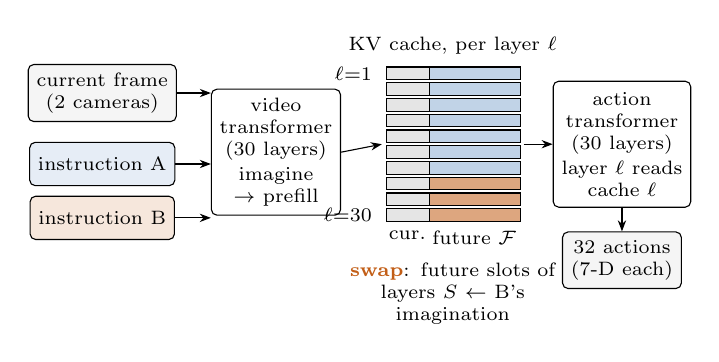
\begin{tikzpicture}[font=\scriptsize, >={Stealth[length=4pt]},
  box/.style={draw, rounded corners=2pt, align=center, inner sep=3pt, minimum height=0.55cm},
  cell/.style={draw, minimum height=0.16cm, inner sep=0pt}]
  % inputs
  \node[box, fill=gray!8] (obs) at (0,0) {current frame\\(2 cameras)};
  \node[box, fill=cA!12, below=0.25cm of obs] (ia) {instruction A};
  \node[box, fill=cB!15, below=0.12cm of ia] (ib) {instruction B};
  % video DiT
  \node[box, minimum width=1.25cm, minimum height=1.6cm, right=0.45cm of ia, yshift=0.15cm] (vdit)
    {video\\transformer\\(30 layers)\\[1pt]imagine\\$\to$ prefill};
  \draw[->] (obs.east) -- (obs.east -| vdit.west);
  \draw[->] (ia.east) -- (ia.east -| vdit.west);
  \draw[->] (ib.east) -- (ib.east -| vdit.west);
  % cache
  \begin{scope}[shift={(3.6,0.25)}]
    \foreach \l in {0,...,9} {
      \pgfmathsetmacro{\y}{-\l*0.2}
      \node[cell, fill=gray!20, minimum width=0.55cm, anchor=west] at (0,\y) {};
      \ifnum\l>6
        \node[cell, fill=cB!55, minimum width=1.15cm, anchor=west] at (0.55,\y) {};
      \else
        \node[cell, fill=cA!30, minimum width=1.15cm, anchor=west] at (0.55,\y) {};
      \fi
    }
    \node[above, align=center] at (0.85,0.12) {KV cache, per layer $\ell$};
    \node[below, align=center] at (0.275,-1.88) {cur.};
    \node[below, align=center] at (1.125,-1.88) {future $\Fut$};
    \node[left, align=right] at (-0.05,-0.0) {$\ell{=}1$};
    \node[left, align=right] at (-0.05,-1.8) {$\ell{=}30$};
  \end{scope}
  \draw[->] (vdit.east) -- (3.55,-0.65);
  % action DiT
  \node[box, minimum width=1.3cm, minimum height=1.6cm] (adit) at (6.6,-0.65)
    {action\\transformer\\(30 layers)\\[1pt]layer $\ell$ reads\\cache $\ell$};
  \draw[->] (5.35,-0.65) -- (adit.west);
  \node[box, fill=gray!8, below=0.3cm of adit] (act) {32 actions\\(7-D each)};
  \draw[->] (adit) -- (act);
  \node[align=center, text width=3.2cm] at (4.45,-2.55) {\textcolor{cB}{\textbf{swap}}: future slots of\\layers $S$ $\leftarrow$ B's imagination};
\end{tikzpicture}
\caption{Fast-WAM's IDM path and our intervention. The video transformer imagines a future clip and is run once more on
the finished clip to fill a key/value (KV) cache at every layer: 98 current-frame tokens and 196 imagined-future tokens
$\Fut$. Action layer $\ell$ attends to cache layer $\ell$. We overwrite the future slots of chosen layers $S$ with those
computed from task~B's imagination (here $S$ = layers 21--30, orange), keeping the current frame and the instruction.}
\label{fig:method}
\end{figure}

\subsection{Fast-WAM}
Fast-WAM~\cite{yuan2026fastwam} pairs the Wan2.2-TI2V-5B video diffusion transformer~\cite{wan2025wan} (30 layers,
width 3072) with a 1B-parameter action transformer (30 layers, width 1024) in a mixture-of-transformers
design~\cite{liang2025mot}: the two networks have separate weights, but at every layer they share one attention
operation (24 heads of dimension 128). The released Optional-IDM checkpoint for LIBERO~\cite{liu2023libero} runs in two
modes from the same weights. In \emph{IDM mode}, the video transformer generates a 9-frame clip by 10 flow-matching
steps~\cite{lipman2022flow,liu2022rectified}, with the current frame clamped; the finished clip is passed through the
video transformer once more to fill a KV cache at every layer; the action transformer then denoises a chunk of 32
seven-dimensional actions (end-effector translation and rotation, gripper) in 10 steps, its layer~$\ell$ attending to
cache layer~$\ell$ and to the other action tokens. In \emph{first-frame mode}, the action reads only the current frame.

Both cameras (224$\times$224 each) are placed side by side and encoded by the video autoencoder, which compresses 16$\times$
in space and 4$\times$ in time; with 2$\times$2 patches, each latent frame becomes 98 tokens (a 7$\times$14 grid, main
camera on the left half). The cache therefore holds 294 tokens per layer: 98 for the current frame and 196, denoted
$\Fut$, for two imagined latent frames. The video attention mask is causal by frame, so current-frame tokens never see
the imagined future; their cache entries do not depend on it. The instruction reaches the action transformer separately,
through cross-attention to text embeddings to which the robot's proprioceptive state is appended.

\subsection{Patching the imagined future}
Let $K^A_\ell, V^A_\ell \in \mathbb{R}^{294\times 3072}$ be the cache of a run imagined with instruction~A, and
$K^B_\ell, V^B_\ell$ the cache computed from a \emph{donor} imagination. For a set of layers $S$ and a mixing weight
$\alpha$, we set
\begin{equation}
\tilde K_\ell[\Fut] = (1-\alpha)\,K^A_\ell[\Fut] + \alpha\,K^B_\ell[\Fut], \quad \ell \in S,
\label{eq:patch}
\end{equation}
and likewise for $V$, leaving all other entries, the instruction and the action noise unchanged. A swap is $\alpha = 1$.
We also replace $\Fut$ with uninformative futures (the mean future over states, Gaussian noise matched in mean and
variance, or the cache of a static clip that repeats the current frame), patch the current-frame slots instead, or
mask attention from actions to $\Fut$ entirely (\emph{knockout}). Finer variants restrict the swap to one imagined frame,
one camera, a subset of tokens, or the 128 channels of a single head.

\textbf{Measures.} Actions are compared in the model's normalized action space (each dimension min-max scaled to
$[-1,1]$). The \emph{action change} is $\Delta = \lVert \hat a' - \hat a \rVert_2$ over all $32\times7$ values between the
edited and unedited action chunks, with identical noise. The \emph{noise floor} is $\Delta$ obtained by resampling only
the action noise. When the donor comes from task~B with its own unedited action $\hat a_B$, the \emph{pull} toward B is
$1-\lVert \hat a'-\hat a_B\rVert / \lVert \hat a-\hat a_B\rVert$ (0: no movement toward B; 1: B's action).

\textbf{Action lens.} With flow matching, the action head predicts a velocity $v$ from which the clean action is
estimated as $\hat x_0 = a_k - \sigma_k v$ at denoising step $k$ with noise level $\sigma_k$. Since the head is a single
linear map, we apply it to the action stream $h_\ell$ after each layer, $\hat x_0^{(\ell)} = a_k - \sigma_k W h_\ell$
(raw lens~\cite{nostalgebraist2020logitlens}), or first map $h_\ell$ to the last layer with a per-layer affine
transform fitted by ridge regression on unedited runs (tuned lens~\cite{belrose2023tuned}). The decoded action is scored
as $d_A/(d_A+d_B)$, its relative distance to the unedited actions for A and for B (0: A, 1: B). We read the lens at the
first denoising step, which starts from the same noise in every run, so differences reflect only the layer's state.

\subsection{Protocol}
\textbf{Validation.} We split the official inference function into imagine, prefill and act stages so that the cache can
be edited. Run unedited, the split pipeline reproduces the official action bit for bit, a self-patch changes nothing,
all checkpoint tensors load without missing keys, and the lens applied to the final layer reproduces the model's
output exactly. Experiments use bf16 on single NVIDIA L40S GPUs (one decision: 0.31\,s imagining, 0.28\,s acting).

\textbf{Tasks and states.} LIBERO-Goal has ten tasks in one kitchen scene (drawers, stove, bowl, plate, wine bottle and
rack, cream cheese), so the goal of any task can be checked on any simulator state. We pair task~A with
B $= (A+5) \bmod 10$ (e.g., ``open the middle drawer of the cabinet'' with ``push the plate to the front of the stove''). Open-loop
analyses use 100 states: first training demonstrations (10 tasks $\times$ 2 episodes $\times$ 5 time points, three seeds),
then 100 fresh states saved from our own closed-loop rollouts (2 decisions from each of 50 episodes), which the model
never trained on; the donor is a state of a different task. Closed-loop runs follow the official evaluation (wait
30 steps, re-plan every 10 steps, 400-step limit) for 10 tasks $\times$ 5 LIBERO starting states, at seed 42 and,
for the main comparison, seeds 0 and 1. At every decision the donor is imagined from the robot's current observation
with B's instruction, and B's goal is checked on the same simulator state. Intervals are 95\% bootstrap over episodes
(open loop) or Wilson intervals (success rates).

% ======================================================================================================
\section{Open Loop: The Action Follows the Imagined Future}
\label{sec:open}

\begin{table}[t]
\centering
\caption{Action change when the imagined future (or the current frame) is replaced in all 30 layers. Training: 100
demonstration states, three seeds. Fresh: 100 states from our rollouts. Noise floor: \nfloorTrain{} / \nfloorFresh.}
\label{tab:open}
\begin{tabular}{@{}lcc@{}}
\toprule
Replacement & Training & Fresh \\
\midrule
Future from another task & \textbf{\nDonorTrain} & \textbf{\nDonorFresh} \\
\quad distance to that task's own action & \nDonorToDonorTrain{} (was \nCleanToDonorTrain) & \nDonorToDonorFresh{} (was \nCleanToDonorFresh) \\
Mean future & \nMeanTrain & \nMeanFresh \\
Static future (current frame repeated) & \nStaticTrain & \nStaticFresh \\
Noise future & \nNoiseTrain & \nNoiseFresh \\
Knockout ($=$ first-frame mode) & \nKnockTrain & \nKnockFresh \\
Current frame from another task & \nPresentTrain & \nPresentFresh \\
\midrule
Other task's future, layers 1--10 & \nBandOneTrain & \nBandOneFresh \\
\phantom{Other task's future,} layers 11--20 & \nBandTwoTrain & \nBandTwoFresh \\
\phantom{Other task's future,} layers 21--30 & \nBandThreeTrain & \nBandThreeFresh \\
\bottomrule
\end{tabular}
\end{table}

\textbf{The action is rewritten by the imagined future.} Replacing the imagined future with one imagined for another
task changes the action by \nDonorFresh{} on fresh states, \nRatioFresh$\times$ the noise floor, and moves it to within
\nDonorToDonorFresh{} of that task's own action, from \nCleanToDonorFresh{} (Table~\ref{tab:open}). Replacing the
current frame instead changes it by only \nPresentFresh. Uninformative futures (mean, static, noise) disturb the action
by a fifth to a half as much without steering it anywhere. Conversely, on demonstrations where the true
future is known, supplying it brings the action to \nTrueToDemo{} from the demonstrated action, against \nCleanToDemo{}
with the model's own imagination: the action pathway behaves as an inverse dynamics reader of whatever future it is
given. Two further observations bear on the test-time debate. Knocking out attention to the future reproduces
first-frame mode exactly, confirming that the two modes differ only in this read. And on demonstrations, first-frame
actions are as close to the demonstrated action as imagine-mode actions (\nFFToDemo{} vs.\ \nCleanToDemo), so the
imagination is not needed for open-loop accuracy, even though it dominates the action when present.

\begin{figure}[t]
\centering
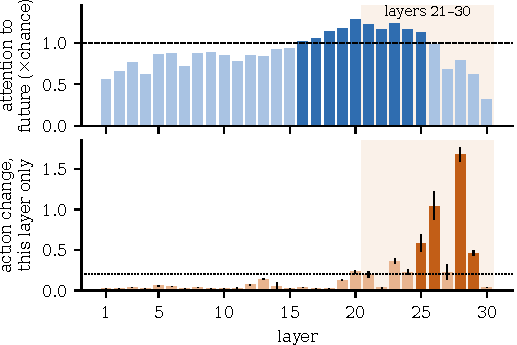
\includegraphics[width=\columnwidth]{figs/attention_vs_use.pdf}
\caption{Attention is not use (fresh states). Top: action-to-future attention per layer, relative to the future's
share of tokens. Bottom: action change when the future is swapped in that layer only; dotted line: noise floor.
Attention peaks around layer \nRfutPeakLayer; the effect sits in layers 25--29.}
\label{fig:attn}
\end{figure}

\textbf{The effect lives in the last ten layers, not where attention peaks.} Swapping the future in layers 1--10 has
no effect (\nBandOneFresh, below the floor), layers 11--20 a small one (\nBandTwoFresh), and layers 21--30 almost the full
effect (\nBandThreeFresh). Swapping single layers locates the largest contributions at layer 28 (\nLTwentyEight) and
26 (\nLTwentySix); single layers sum to \nSingleSum, short of the all-layer \nDonorFresh, so layers act jointly
(Fig.~\ref{fig:attn}). We recorded the attention weights in the same runs, recomputing them in full precision (the
grouped outputs reconstruct the model's attention output to within $\nReconErr$). Action tokens give 19--77\% of their
attention to the future in every layer, and more than its token share only in layers 16--25 (peak \nRfutPeak$\times$ at
layer \nRfutPeakLayer); layers 27--30 attend mostly to the other action tokens (\nMactLateLo--\nMactLateHi). The
layers that attend most to the future are thus not the ones whose future the action depends on, a dissociation of the
kind cautioned against in~\cite{jain2019attention}. All results replicate between training and fresh states.

% ======================================================================================================
\section{Closed Loop: The Robot Does What It Imagines}
\label{sec:closed}

\begin{figure}[t]
\centering
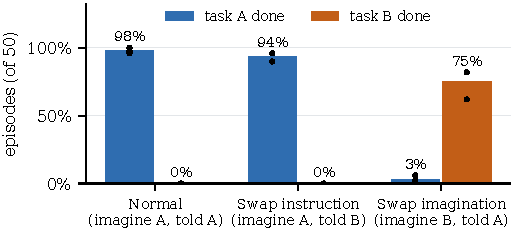
\includegraphics[width=\columnwidth]{figs/flip_seeds.pdf}
\caption{Closed loop, 10 tasks $\times$ 5 starting states $\times$ 3 seeds. Bars: mean over seeds; dots: individual
seeds. ``Done'' means the task's goal was satisfied in the simulator.}
\label{fig:flip}
\end{figure}

We now apply Eq.~\eqref{eq:patch} at every decision of a full episode. In the normal policy the robot completes task~A in
\nCleanAPooled{} of 150 episodes. If the action transformer is told B while the cache holds A's imagination, it still
completes A in \nTextAPooled{} of 150 episodes (\nTextASeeds{} per seed) and never B. If instead the cache holds B's
imagined future while the action is told A, the robot completes A in \nFutAPooled{} episodes and B in
\nFutBPooled{} (\nFutBSeeds{} per seed; Fig.~\ref{fig:flip}). It does so fluently: B's goal is reached after a median of
\nMedStepsFutB{} steps, against \nMedStepsClean{} for A in normal runs. B's goal check never fired in normal or
instruction-swapped runs (0/300). The robot does not merely fail task~A; it performs the task it imagines. The
instruction still matters, through the imagination it produces, but given a fixed imagined future the action
transformer's own access to the instruction has no measurable effect.

\begin{figure}[t]
\centering
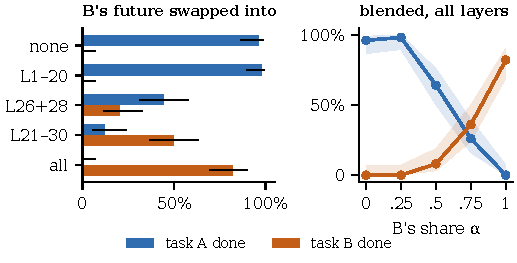
\includegraphics[width=\columnwidth]{figs/localize_dose.pdf}
\caption{Closed loop, seed 42, 50 episodes per row or point. Left: B's future swapped into some layers only; the rest
keep A's. Right: futures blended in all layers, Eq.~\eqref{eq:patch}. Error bars and bands: 95\% Wilson intervals.}
\label{fig:localize}
\end{figure}

\textbf{Late layers are sufficient; early layers are not.} Restricting the swap to layers 1--20 leaves behavior intact
(A \nBandEarlyA\%, B \nBandEarlyB\%). Restricting it to layers 21--30 suppresses task~A (\nBandLateA\%) and produces
B in \nBandLateB\% of episodes; layers 26 and 28 alone, the two strongest single layers, do part of this (A
\nBandTwoLayersA\%, B \nBandTwoLayersB\%; Fig.~\ref{fig:localize}, left). Episodes that end in neither goal show mixed
behavior; for example, with the late layers swapped, a robot told to put the bowl on top of the cabinet while imagining putting
the wine bottle on the rack picked up the bowl, set it down on the stove instead, and stayed there until the time limit.

\textbf{A threshold, not a linear dial.} Blending the two futures (Fig.~\ref{fig:localize}, right) leaves behavior
unchanged at $\alpha = 0.25$ (A \nAlphaQA\%), mixed at $0.5$ (A \nAlphaHA\%, B \nAlphaHB\%), and mostly flipped at
$0.75$ (A \nAlphaTQA\%, B \nAlphaTQB\%). A minority share of a foreign future is ignored; the policy commits once
the foreign future dominates.

% ======================================================================================================
\section{Mechanism: What Is Read, and Where It Is Decided}
\label{sec:mech}

\begin{table}[t]
\centering
\caption{Partial swaps of another task's imagined future (all layers, 100 fresh states). Pull: fraction of the way
from the unedited action to the other task's action.}
\label{tab:parts}
\begin{tabular}{@{}lcc@{}}
\toprule
Swapped part of the future & Change & Pull \\
\midrule
All 196 tokens & \nPAll & \nPAllPull \\
50\% of tokens that differ most & \textbf{\nPTop} & \textbf{\nPTopPull} \\
Random 50\% of tokens & \nPRand & \nPRandPull \\
50\% of tokens that differ least & \nPBottom & \nPBottomPull \\
Imagined frame 1 / frame 2 & \nPFOne{} / \nPFTwo & \nPFOnePull{} / \nPFTwoPull \\
Main camera / wrist camera & \nPMain{} / \nPWrist & \nPMainPull{} / \nPWristPull \\
\bottomrule
\end{tabular}
\end{table}

\textbf{What is read: where the futures differ.} We rank the 196 future tokens by how much the two imagined latent
videos differ at each position and swap a fraction of them (Table~\ref{tab:parts}). The half that differs most carries
almost the full flip (pull \nPTopPull{} vs.\ \nPAllPull); the half that differs least has nearly no effect
(\nPBottom), and a random half falls in between. The action thus reads the content that distinguishes one imagined
outcome from another, such as the moving arm and objects, rather than the static scene. Neither imagined frame alone and
neither camera alone suffices, and the wrist camera carries more than the main camera (pull \nPWristPull{} vs.\
\nPMainPull).

\begin{figure}[t]
\centering
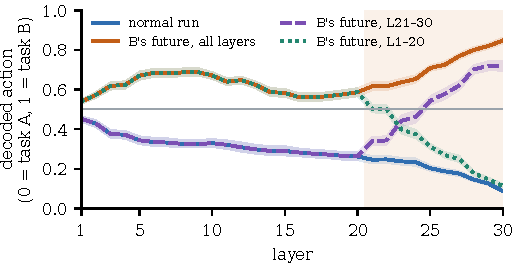
\includegraphics[width=\columnwidth]{figs/action_lens.pdf}
\caption{Tuned action lens on 50 held-out fresh states (the lens was fitted on the other 50). Each curve: the action
decoded after each layer, scored between task A (0) and task B (1); bands: 95\% intervals over states.}
\label{fig:lens}
\end{figure}

\textbf{Where it is decided: early layers read, late layers decide.} The tuned action lens (Fig.~\ref{fig:lens}) shows
that when every layer sees B's future, the decoded action already leans toward B by layer 9 (\nLensEarlyNine). This
explains the strong early attention: information about the imagined future does enter early. Yet when only layers 1--20
see B's future, the decoded action leans toward B up to layer 20 (\nLensEarlyTwenty), exactly as in the full swap, and
is then pulled back to A by layers 21--30, which see A's future (\nLensEarlyThirty{} at the output, against
\nLensCleanThirty{} for the unedited run). When only layers 21--30 see B's future, the reverse happens: the action
decodes as A until layer 20 (\nLensLateTwenty) and moves to B afterward (\nLensLateThirty). The late layers therefore
form the decision and override what earlier layers concluded, which reconciles the attention profile with the patching
and closed-loop results. The raw lens, without a learned correction, shows the same late transition but no early signal,
so the early reading is present but not in the output basis.

\textbf{Which heads.} Swapping the future in a single head of layer 26 or 28 identifies a few heads that carry most of
each layer's effect (layer 26: \nHeadTopA; layer 28: \nHeadTopB). No single head moves the action more than
\nHeadMaxPull{} of the way toward B, and a head's attention to the future predicts its effect only moderately
(correlation \nHeadCorrA{} and \nHeadCorrB). The read is thus distributed over a handful of heads in several late layers
rather than concentrated in one ``imagination head''.

% ======================================================================================================
\section{Discussion}

\textbf{Imagination as a control channel.} In this WAM, what the policy imagines determines what it does, more than
what it is told. This has two sides. It is a risk: anything that corrupts the imagined future, whether a generation
failure, a distribution shift in the video model, or an adversarial edit, redirects the robot to a coherent but wrong
task, and the instruction does not act as a safeguard. It is also an opportunity: the imagined video is a readable
forecast of the policy's next behavior, which can be inspected before execution, and the late layers and few heads we
identify are natural targets for monitoring and for steering methods such as~\cite{hong2026steering}. Adversarial
attacks have been shown to decouple a WAM's actions from its imagination~\cite{li2026badwam} or to corrupt the
imagination of imagine-then-act models~\cite{chen2026trusted}; our results show that when the imagination is
coherent but wrong, the action follows it.

\textbf{On the test-time debate.} Our results are compatible with Fast-WAM's finding that imagination is not required
for success~\cite{yuan2026fastwam}: in open loop, first-frame actions are as accurate as imagine-mode actions. They add
that when imagination is present, it is not ignored; it dominates the action. Success rates alone cannot distinguish
these situations. How much a WAM depends on its future also varies with design: masking the future collapses success
in a jointly denoising Fast-WAM variant~\cite{zhang2026rift}, whereas in the Optional-IDM checkpoint masking reproduces
the first-frame mode it was also trained for. Whether imagination helps under harder or perturbed conditions, the claim of~\cite{li2026lawa}, is a
question our patching protocol can address directly.

\textbf{Limitations.} We study one WAM whose action transformer is trained as an inverse dynamics reader, so reliance on
the future is encouraged by design; that it nonetheless ignores its own instruction access, and how and where the
future is read, are not implied by the design, but other WAM architectures, in which video and actions are denoised
jointly, need the same test. Our closed-loop evidence covers one LIBERO suite with ten tasks in one scene, five starting
states per task and three seeds, in simulation; real-robot validation is future work. The B goal is checked every ten
steps. The lens shows what is decodable, not what is used; the claim that late layers decide rests on the patching and
closed-loop experiments, which agree with it.

\section{Conclusion}

We asked whether a world action model acts on what it imagines and answered by intervening on the imagined future
inside the model. In Fast-WAM, it does: the imagined future rewrites the action, and in closed loop the robot carries out
the task it imagines rather than the task it is told. The information enters early but is decided in the last ten
layers, read from the tokens where imagined outcomes differ, through a few heads. Patching the imagined future gives a
direct, causal tool for evaluating, monitoring and steering video-based robot policies.

\section*{Statements}
\textbf{Data and code availability.} Code, per-episode results, analysis scripts and videos are available at
\url{https://github.com/TusharBajaj07/wam-imagination-patching}. The model checkpoint and LIBERO data are public~\cite{yuan2026fastwam,liu2023libero}.
\textbf{Author contributions.}
T.B.: conceptualization, methodology, investigation, analysis, writing.
\textbf{Use of AI tools.} Experiment code, analysis and an initial draft of this paper were prepared with assistance
from an AI system (Claude, Anthropic). The author reviewed all code, results and text and takes full responsibility
for them.
\textbf{Funding and competing interests.} This work received no external funding. The author declares no competing interests.

\bibliographystyle{IEEEtran}
\bibliography{refs}

\end{document}
